%!TEX root = ../paper.tex
\section{Natural User Interface}
\label{sec:nui}

% Warum? Bezug zum Gesamtkozept? Welches Problem löse ich?

% Motivation: Freie Bewegung -> Freihändige Interaktion
In der bisherigen Arbeit wurde bereits das Konzept der freien Bewegung um den Tisch und damit auch um das Modell
vorgestellt. Der Nutzer hat die Möglichkeit, das Modell von allen Seiten zu betrachten. Dies legt nahe, dass auch seine
Interaktion mit dem System möglichst frei sein muss.
% direkte Interaktion, kein Mapping
Dabei wird bewusst auf ein Mapping von 2D-Eingabegeräten auf den virtuellen Raum verzichtet und es wird stattdessen eine
direkte Interaktion angeboten. Der Nutzer hat die Möglichkeit durch Gesten und Tangibles mit dem System zu interagieren.

% Interaktion mit virtuellen Objekte auf gleiche Weise wie Arbeit mit Tangibles (vielleicht)
\todo[inline,color=green!40]{Tangibles zuvor einführen?}
Die Interaktion mit virtuellen Objekten soll auf die gleich Weise möglich sein, wie die Arbeit mit Tangibles. Nutzer
können virtuelle Objekte verschieben, anheben und greifen. Für diesen Zweck werden physikbasierte Gesten verwendet.
% Kombination mit semantisch interpretierten Gesten (Zoomen)
Als zweite Möglichkeit der Nutzung von Gesten zur Interaktion wird eine semantischen Interpretation von Gesten
durchgeführt. Somit ist es möglich, einzelne virtuelle Objekte und die gesamte Szene zu skalieren oder zu rotieren.
In Kombination mit den physikbasierten Gesten wird dem Nutzer eine große Möglichkeit zur Interaktion geboten.
% komplexe Interaktion durch Menüführung vereinfacht
Komplexere Interaktionsformen werden durch den Einsatz einer Menüführung vereinfacht. Damit soll vermieden werden, dass
ein Nutzer sich komplizierte Bewegungsfolgen merken und durchführen muss, um eine gewünschte Aktion auszuführen.


Die Skeletterkennung mit der Kinect wird in vielen wissenschaftlichen Arbeiten behandelt und funktioniert unter guten
Laborbedingungen zuverlässig. Für genauere Operationen wird jedoch eine gute Handerkennung benötigt, welche mit der
Kinect problematisch zu realisieren ist. Aus diesem Grund wird ein zusätzliches Eingabegerät benötigt, mit dem die
Hände der Nutzer erkannt werden können. Die Leap Motion bietet solch eine Funktionalität und arbeitet mit einem
optischen Verfahren. Jedoch wird bei Devices, die sich auf die Erkennung der Hände spezialisiert haben, das restliche
Skelett nicht ermittelt und neben den Händen im besten Fall noch die Ellenbogen zur Verfügung gestellt.
Ideal wäre die gleichzeitige Verwendung einer Kinect oder einem Gerät mit ähnlicher Funktionalität zusammen mit einer
Leap Motion. Für die Verarbeitung dieses Multisensor-Inputs wird die Sensorabstraktion Trame verwendet, wie in Abbildung
\ref{fig:gesture_recognition} zusehen ist.


Dieser Abschnitt erläutert die technische Umsetzung der beiden Subsysteme, die für die Unterstützung von Tangibles und
Gesten verantwortlich sind. 

% Wo wollen wir hin und wie löse ich die Probleme % Was machen andere?
\subsection{Tangible-Tracking}

Im Gegensatz zu dem allgemeinen Verständnis von Tangibles, bei dem sie als ein Eingabecontroller fungieren, werden
Tangibles in dieser Arbeit als reale Objekte angesehen, die Teil der Konstruktion werden. Somit ist das
Tangible-Tracking ein Objekttracking. Zur Erstellung eines Prototypen wurde eine markerbasierte Lösung implementiert.

{\em Aktueller Stand: } Der markerbasierte Ansatz verwendet Würfel als Repräsentation von domänspezifischen Objekten,
z.B. Komponenten einer Murmelbahn. Würfel besitzen eindeutige, rotationsinvariante Marker auf jeder Seite. Es wird eine
2D-Video-Kamera genutzt, um die Marker kontinuierlich zu tracken und die Position der Marker zu ermitteln. Aufgrund der
Eindeutigkeit und Rotationsinvarianz der Marker kann die grobe Ausrichtung und die Identität ermittelt werden. Ein
koplanarer POSIT-Algorithmus\cite{oberkampf1996iterative} wird genutzt um die Position und Rotation des Markers relativ
zur Kamera zu schätzen. Zum Schluss wird die aktuelle Position und Rotation des Würfels im Weltkoordinatensystem
berechnet.


Die Lösung ist in der Lage, bis zu fünf unterschiedliche Objekte in einem Bereich von 0,8 m vor der Kamera mit einer
Aktualisierungsrate von 50 Events pro Sekunde zu erkennen. Dabei wird eine Überdeckung der Marker nicht behandelt.

\subsection{Gestenerkennung}

{\em Konzept:} Das Subsystem zur Gestenerkennung besteht aus zwei Hauptkomponenten: (1) Trame, einer Komponente zur
Geräteabstraktion, um Input von mehreren Sensoren zu verarbeiten und (2) die Erkennungskomponente zur Gestenerkennung,
wie in Abbildung \ref{fig:gesture_recognition} zu sehen ist. Trame transformiert Sensordaten in ein einheitliches
Skelettformat. Die Gestenerkennung teilt sich in eine Pipeline für die Berechnung physikbasierter Gesten und eine
Pipeline für die Interpretation von Gesten. Die gemeinsame Vorverarbeitung der Skelette wird genutzt um Wackler zu
entfernen sowie die Hand- und Armpositionen zu ermitteln.

\begin{figure}[H]
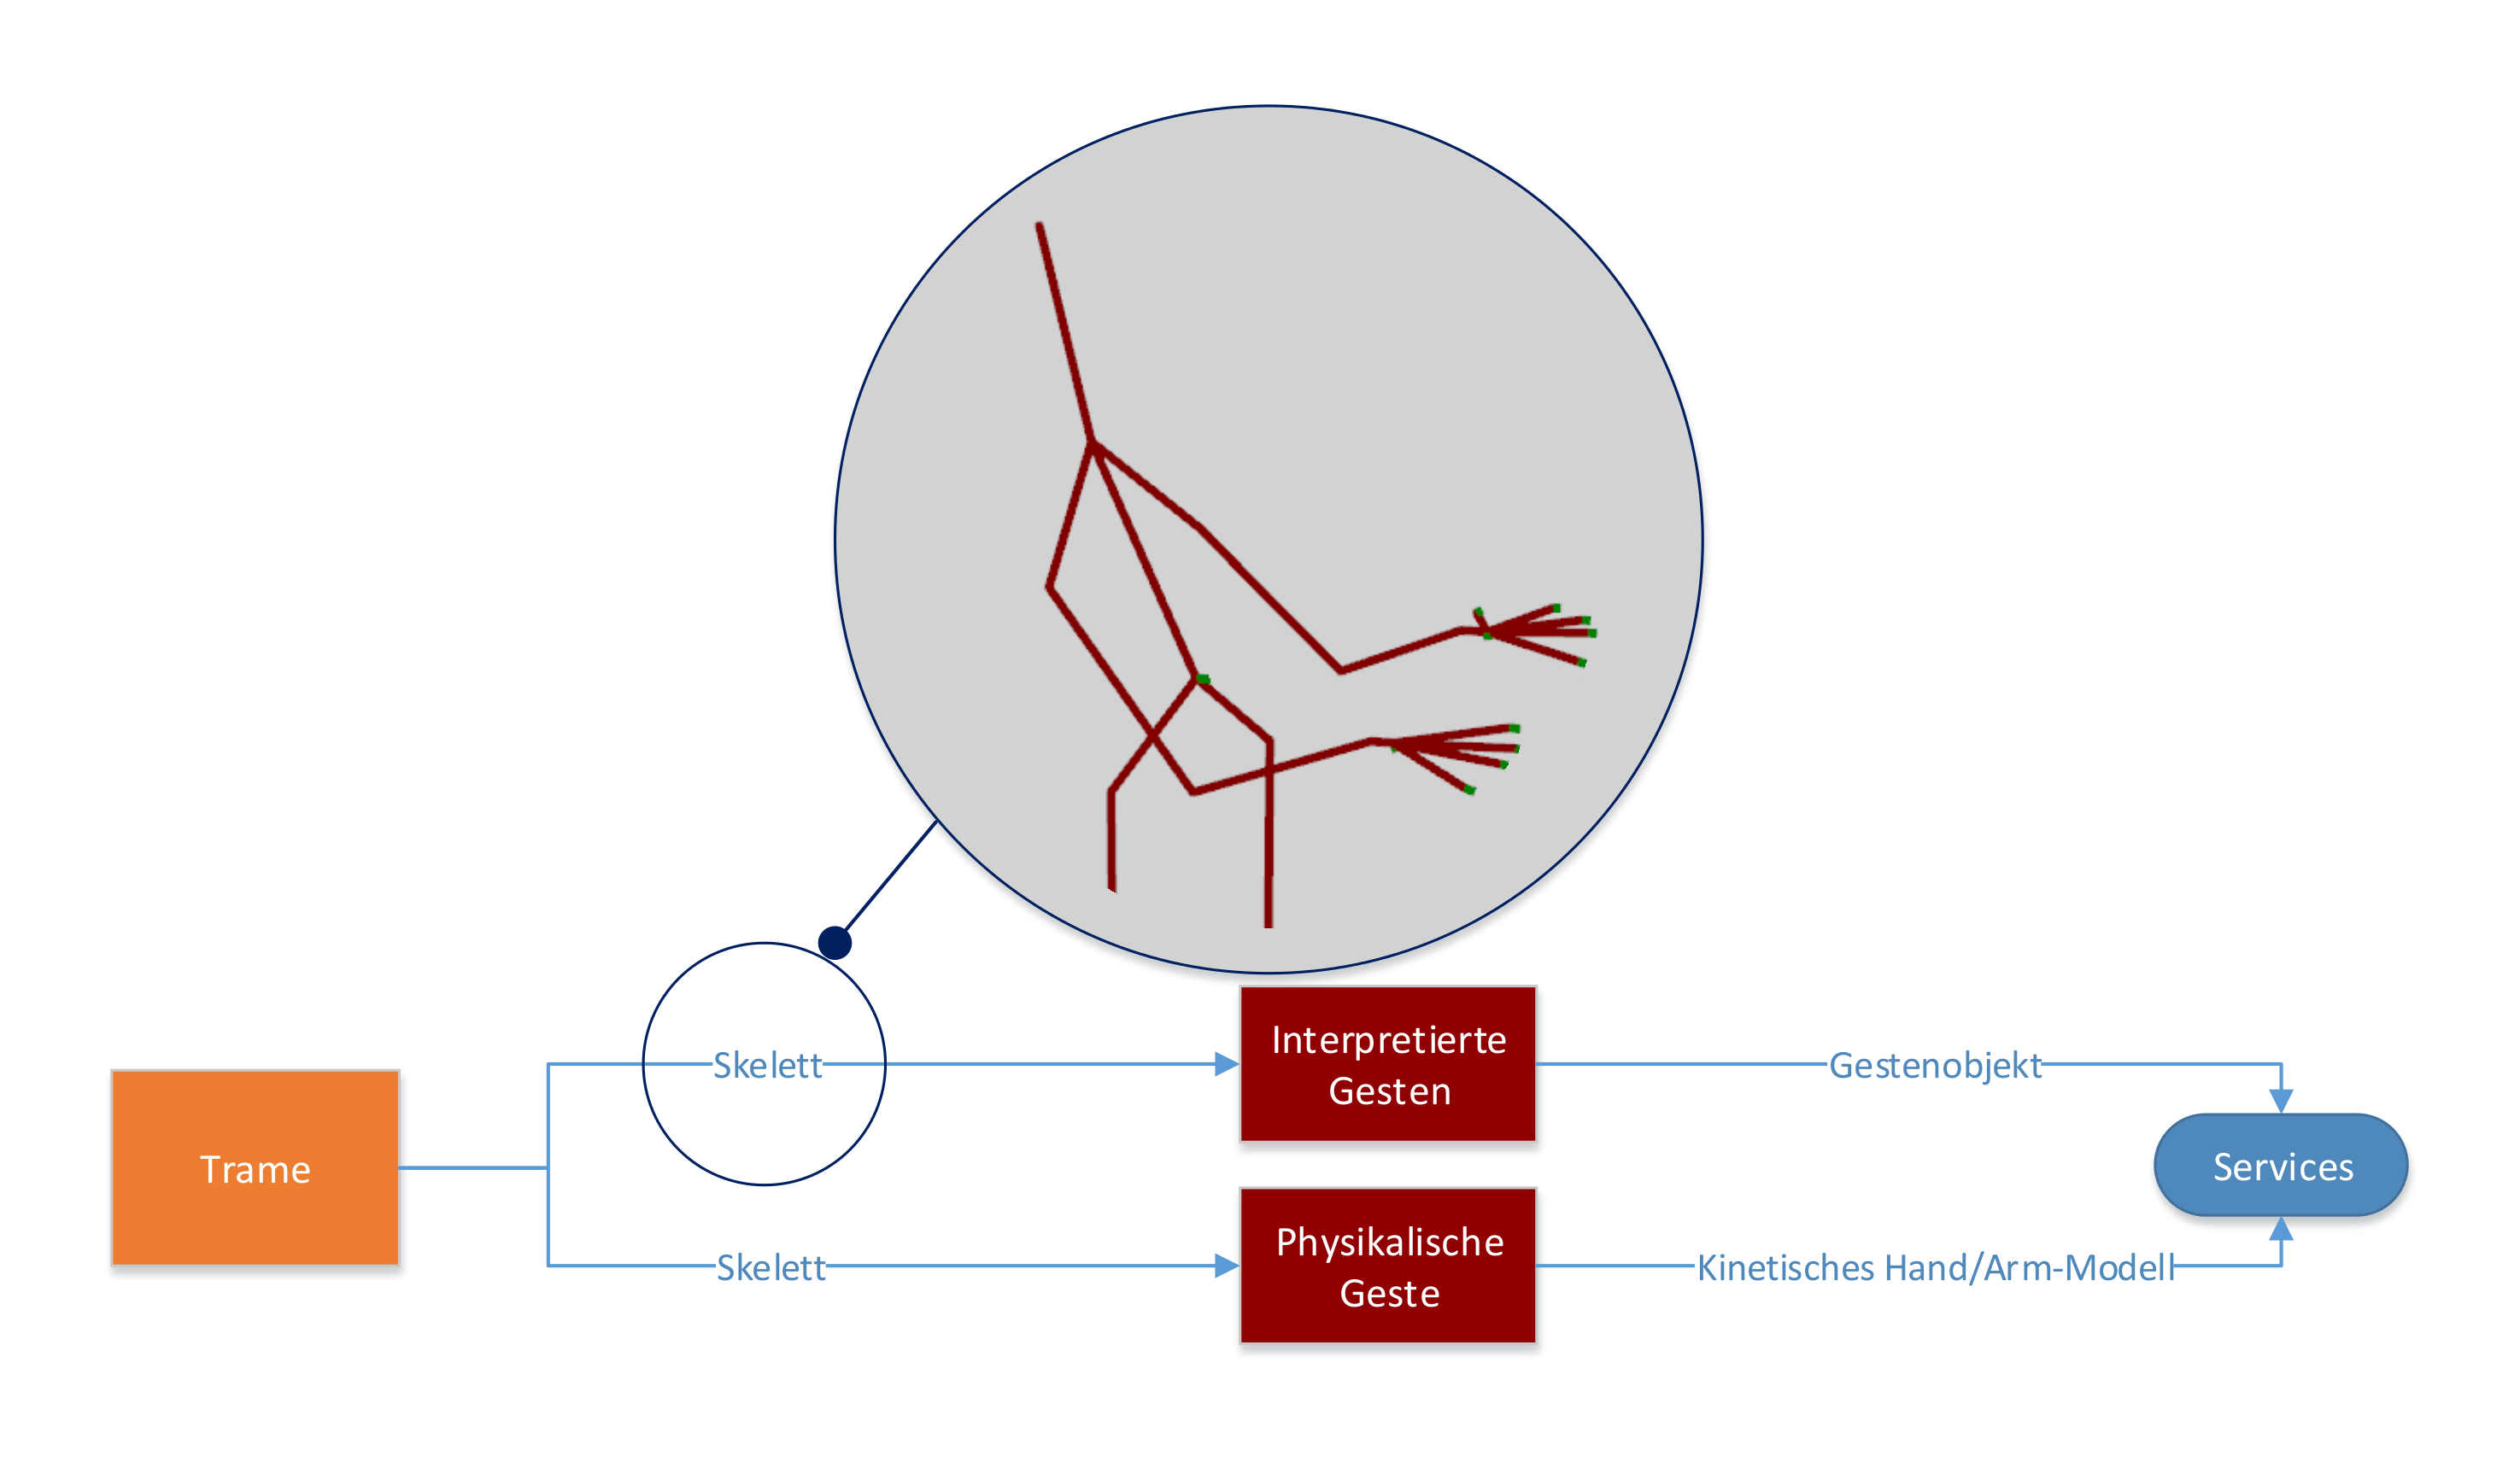
\includegraphics[width=\columnwidth]{figs/gesture_recognition_pipeline}
\caption{Übersicht des Modules für gestenbasierte Interaktion mit Device-Abstaktions und Gestenerkennung.}
\label{fig:gesture_recognition}
\end{figure}

Templatematching\cite{Kristensson:2012:CRO:2166966.2166983} erweitert um die Einbeziehung der dritten Dimension und eine
Erweiterung der Eingabepunkte ist für die Erkennung von interpretierten Gesten verantwortlich. Parallel dazu wird ein
Collider-Objekt berechnet, dass Hand- und Armbewegungen darstellt, um physikalische Gesten einzubeziehen. Im 
Entscheidungsschritt können interpretierte Gesten entsprechende Events auslösen, welche in die Umgebung verteilt werden.
In jedem Fall wird ein Collider-Objekt zur Weiterverarbeitung bereitgestellt. 


{\em Aktueller Status:} Trame wurde implementiert und getestet. Auch die Gestenverarbeitung ist implementiert, aber
noch nicht getestet worden. 


{\em Nächste Schritte:} Es muss ein Gestenset definiert werden, durch das ein Nutzer interagieren kann. Nach
ausführlichen Tests sollen Usability-Studien durchgeführt werden, um die Hauptannahme zu verifizieren, das die
Bereitstellung von physikalischen und interpretierten Gesten dem Nutzer eine Schnittstelle bietet,
mit der er schnell und natürlich interagieren kann.